\newpage
\section{Ôn tập Chương 3}
\def\thoigian{90}%--Thời gian
\de{Đề số 1}{Chương III. Hàm số bậc hai và đồ thị}
\begin{center}
	\textbf{PHẦN 1 - CÂU TRẮC NGHIỆM BỐN PHƯƠNG ÁN}
\end{center}
\Opensolutionfile{ans}[ans/ans-TN-ONTAPCHUONG-DE1]
\begin{ex}%[Dự án đề cương 3 khối 10-11-12 Dot 3 -Truong Tuong]
	Xét hai đại lượng $x$ và $y$ phụ thuộc vào nhau theo các hệ thức dưới đây. Trường hợp nào thì $y$ \textbf{không phải} là hàm số của $x$? 
	\choice
	{$y$ là số vụ tại nạn xảy ra trên một tuyến đường vào ngày thứ $x$ trong tháng 12/2025}
	{$y$ là số học sinh của một lớp vắng học vào ngày thứ $x$ trong tuần}
	{$y$ là số lượng học sinh của một lớp có điểm số $x$ trong bài kiểm tra}
	{\True $y$ là điểm số có $x$ học sinh của một lớp đạt được trong bài kiểm tra}
	\loigiai{
		Nếu $y$ là điểm số có $x$ học sinh của một lớp đạt được trong bài kiểm tra thì với mỗi giá trị $x$ có thể xác định được nhiều hơn một giá trị $y$. \\
		Ví dụ, có thể có $5$ học sinh ($x=5$) đạt $8$ điểm và cũng có $5$ học sinh đạt $9$ điểm, tức là với $x=5$ thì $y=8$ hoặc $y=9$. \\
		Do đó $y$ không phải là hàm số của $x$. 
	}
\end{ex}
\begin{ex}%[Dự án đề cương 3 khối 10-11-12 Dot 3 -Truong Tuong]
	Tìm tập xác định $\mathscr{D}$ của hàm số $y=\sqrt{2x-4}$.
	\choice
	{$(2;+\infty)$}
	{$(-\infty;2)$}
	{\True $[2;+\infty)$}
	{$(-\infty;2]$}
	\loigiai{
		Hàm số $y$ xác định khi $2x-4 \ge 0$ hay $x \ge 2$. \\
		Vậy tập xác định $\mathscr{D}=[2;+\infty)$.
	}
\end{ex}
\begin{ex}%[Dự án đề cương 3 khối 10-11-12 Dot 3 -Truong Tuong]
	Cho hàm số $f(x)=\dfrac{2x-3}{x+1}$. Tính giá trị của hàm số đã cho tại điểm $x=-2$. 
	\choice
	{$-5$}
	{$5$}
	{\True $7$}
	{$-7$}
	\loigiai{
		Ta có $f(-2)=\dfrac{2 \cdot (-2)-3}{-2+1}=7$.
	}
\end{ex}
\begin{ex}%[Dự án đề cương 3 khối 10-11-12 Dot 3 -Truong Tuong]
	Tìm tất cả các khoảng nghịch biến của hàm số $y=-x^2+2x-3$.
	\choice
	{$(-\infty;1)$}
	{\True $(1;+\infty)$}
	{$(-2;+\infty)$}
	{$(-\infty;2)$}
	\loigiai{
		Có $a=-1<0$ và $b=2$. \\
		Suy ra $-\dfrac{b}{2a}=1$. \\
		Hàm số $y=-x^2+2x-3$ nghịch biến trên khoảng $(1;+\infty)$.
	}
\end{ex}
\begin{ex}%[Dự án đề cương 3 khối 10-11-12 Dot 3 -Truong Tuong]
	Tọa độ đỉnh của đồ thị hàm số $y=2x^2+5x-1$ là
	\choice
	{\True $\left(-\dfrac{5}{4};-\dfrac{33}{8}\right)$}
	{$\left(-\dfrac{5}{2};-1\right)$}
	{$\left(\dfrac{5}{4};\dfrac{67}{8}\right)$}
	{$\left(-\dfrac{5}{4};-1\right)$}
	\loigiai{
		Tọa độ đỉnh của đồ thị hàm số $y=2x^2+5x-1$ là $\left(-\dfrac{5}{4};-\dfrac{33}{8}\right)$.
	}
\end{ex}
\begin{ex}%[Dự án đề cương 3 khối 10-11-12 Dot 3 -Truong Tuong]
	\immini{
		Cho hàm số bậc hai có đồ thị như hình bên. Hàm số đã cho đạt giá trị nhỏ nhất tại điểm nào sau đây?
		\choice[1]
		{$x=-2$}
		{\True $x=2$}
		{$y=-2$}
		{$y=2$}
	}
	{
		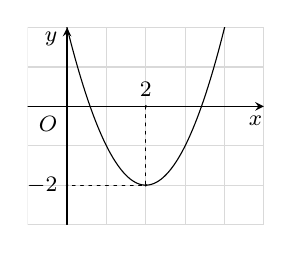
\begin{tikzpicture}[scale=0.5,>=stealth,line join=round,line cap=round,font=\footnotesize]
			\def\xmin{-1} 
			\def\xmax{5}
			\def\ymin{-3} 
			\def\ymax{2} 
			\clip (\xmin,\ymin) rectangle (\xmax,\ymax);
			\draw [gray!30] (\xmin,\ymin) grid (\xmax,\ymax);
			\draw [smooth, samples=100] plot [domain=\xmin:\xmax] (\x,{(\x-2)^2-2});
			\draw [->] (\xmin,0)--(\xmax,0) node [below, xshift=-3pt] {$x$};
			\draw [->] (0,\ymin)--(0,\ymax) node [left, yshift=-4pt] {$y$};
			\draw [dash pattern=on 1pt off 2pt] (2,0)--(2,-2)--(0,-2);
			\fill [black] (0,0) circle (1pt) node [below left] {$O$}
			(2,0) circle (1pt) node [above] {$2$}
			(0,-2) circle (1pt) node [left] {$-2$}
			(2,-2) circle (1pt);
		\end{tikzpicture}
	}
	\loigiai{
		Từ đồ thị ta có: hàm số đạt giá trị nhỏ nhất tại điểm $x=2$.
	}
\end{ex}
\begin{ex}%[Dự án đề cương 3 khối 10-11-12 Dot 3 -Truong Tuong]
	Tìm tập giá trị của hàm số $y=\sqrt{4-2x}$.
	\choice
	{$(2;+\infty)$}
	{$(0;+\infty)$}
	{\True $[0;+\infty)$}
	{$(-\infty;2]$}
	\loigiai{
		Tập xác định của hàm số là $\mathscr{D}=(-\infty;2]$. \\
		Với mọi $x \in \mathscr{D}$ thì $y=\sqrt{4-2x} \ge 0$. \\
		Vậy tập giá trị của hàm số đã cho là $[0;+\infty)$.
	}
\end{ex}
\begin{ex}%[Dự án đề cương 3 khối 10-11-12 Dot 3 -Truong Tuong]
	\immini{
		Cho hàm số $y=f(x)$ có đồ thị như hình bên. Tìm tất cả giá trị của $x$ để $y=2$? 
		\motcot
		{$x=-2$, $x=2$}
		{$x=-1$, $x=1$}
		{$x=-1$, $x=3$}
		{\True $x=-3$, $x=1$}
	}
	{
		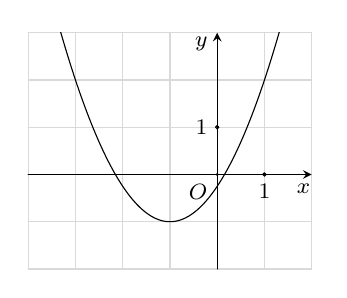
\begin{tikzpicture}[scale=0.6, >=stealth, line join=round, line cap=round, font=\footnotesize]
			\def\xmin{-4} 
			\def\xmax{2}
			\def\ymin{-2} 
			\def\ymax{3} 
			\draw[gray!30] (\xmin,\ymin) grid (\xmax,\ymax);
			\draw [->] (\xmin,0)--(\xmax,0) node [below, xshift=-3pt] {$x$};
			\draw [->] (0,\ymin)--(0,\ymax) node [left, yshift=-4pt] {$y$};
			\fill [black] (0,0) circle (1pt) node [below left] {$O$};
			\clip (\xmin,\ymin) rectangle (\xmax,\ymax);
			\draw[smooth, samples=100] plot [domain=\xmin:\xmax] ({\x},{0.75*(\x)^2+1.5*(\x)-0.25});
			\draw (1,0) circle (1 pt) node [below] {$1$}
			(0,1) circle (1pt) node [left] {$1$};
		\end{tikzpicture}
	}
	\loigiai{
		\immini{
			Đường thẳng $y=2$ cắt đồ thị hàm số đã cho tại hai điểm phân biệt có hoành độ là $x=-3$, $x=1$. \\
			Vậy để $y=2$ thì $x=-3$, $x=1$. 
		}
		{
			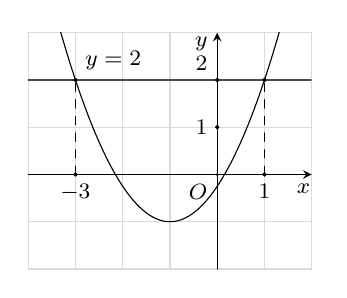
\begin{tikzpicture}[scale=0.6, >=stealth, line join=round, line cap=round, font=\footnotesize]
				\def\xmin{-4} 
				\def\xmax{2}
				\def\ymin{-2} 
				\def\ymax{3} 
				\draw[gray!30] (\xmin,\ymin) grid (\xmax,\ymax);
				\draw [->] (\xmin,0)--(\xmax,0) node [below, xshift=-3pt] {$x$};
				\draw [->] (0,\ymin)--(0,\ymax) node [left, yshift=-4pt] {$y$};
				\fill [black] (0,0) circle (1pt) node [below left] {$O$};
				\clip (\xmin,\ymin) rectangle (\xmax,\ymax);
				\draw [smooth, samples=100] plot [domain=\xmin:\xmax] ({\x},{0.75*(\x)^2+1.5*(\x)-0.25})
				(\xmin,2)--(\xmax,2) node [above, pos=.3] {$y=2$};
				\draw [dashed] (-3,0)--(-3,2) (1,0)--(1,2);
				\draw [fill=black] (1,0) circle (1 pt) node [below] {$1$} 
				(0,2) circle (1pt) node [above left] {$2$}
				(-3,0) circle (1pt) node [below] {$-3$}
				(-3,2) circle (1pt) (1,2) circle (1pt)
				(0,1) circle (1pt) node [left] {$1$};
			\end{tikzpicture}
		}
	}
\end{ex}
\begin{ex}%[Dự án đề cương 3 khối 10-11-12 Dot 3 -Truong Tuong]
	Tìm tập xác định của hàm số $y=\dfrac{2x-1}{\sqrt{3-x}}$.
	\choice
	{$\mathscr{D}=[3;+\infty)$}
	{$\mathscr{D}=(3;+\infty)$}
	{$\mathscr{D}=(-\infty;3]$}
	{\True $\mathscr{D}=(-\infty;3)$}
	\loigiai{
		Hàm số đã cho xác định khi $3-x>0$ hay $x<3$. \\
		Vậy tập xác định của hàm số là $\mathscr{D}=(-\infty;3)$.
	}
\end{ex}
\begin{ex}%[Dự án đề cương 3 khối 10-11-12 Dot 3 -Truong Tuong]
	Cho hàm số $y=2x^2-(m+1)x-3$ ($m \in \mathbb{R}$). Biết đồ thị hàm số đã cho có hoành độ đỉnh bằng $3$. Tìm $m$.
	\choice
	{\True $m=11$}
	{$m=4$}
	{$m=-3$}
	{$m=5$}
	\loigiai{
		Đồ thị hàm số đã cho có hoành độ đỉnh là $x=\dfrac{m+1}{4}$. \\
		Theo đề ta có $\dfrac{m+1}{4}=3$ hay $m=11$.
	}
\end{ex}
\begin{ex}%[Dự án đề cương 3 khối 10-11-12 Dot 3 -Truong Tuong]
	\immini{
		Một đất hình chữ nhật có chiều rộng bằng $x$ m và chiều dài gấp đôi chiều rộng. Người ta mở rộng mảnh đất đó bằng cách tăng chiều dài thêm $2$ m và tăng chiều rộng thêm $1$ m như hình bên. Diện tích (đơn vị: $\text{m}^2$) của mảnh đất mới được biểu diễn bởi hàm số bậc hai nào sau đây?
		\choice [2]
		{$S(x)=2x^2+2x+2$}
		{\True $S(x)=2x^2+4x+2$}
		{$S(x)=2x^2+4x+1$}
		{$S(x)=2x^2+4$}
	}
	{
		\begin{tikzpicture}[scale=0.7,>=stealth,line join=round,line cap=round,font=\footnotesize]
			\draw (0,0)--++(5,0)--++(90:2.5)--++(180:5)--cycle node [left, pos=.5] {$x$ m};
			\draw [dashed] (5,0)--++(2,0) node [above, pos=.5] {$2$ m}--++(0,3.5)--++(180:7)--++(-90:1) node [left, pos=.5] {$1$ m};
		\end{tikzpicture}
	}
	\loigiai{
		Chiều rộng của mảnh đất mới là $x+1$ (m). \\
		Chiều dài của mảnh đất mới là $2x+2$ (m). \\
		Diện tích của mảnh đất mới là $S(x)=(x+1) \cdot (2x+2)=2x^2+4x+2$ $\left(\text{m}^2\right)$.
	}
\end{ex}
\begin{ex}%[Dự án đề cương 3 khối 10-11-12 Dot 3 -Truong Tuong]
	\immini{
		Cho hàm số bậc hai $y=ax^2+bx+c$ có đồ thị như hình bên. Mệnh đề nào sau đây là đúng?
		\choice[1]
		{$a<0, \; b>0, \; c<0$}
		{\True $a<0, \; b>0, \; c>0$}
		{$a<0, \; b<0, \; c<0$}
		{$a>0, \; b>0, \; c>0$}
	}
	{
		\begin{tikzpicture}[scale=0.55, x=1cm, y=1cm, line join=round, line cap=round,>=stealth]
			\def\xmin{-2}
			\def\xmax{4}
			\def\ymin{-2}
			\def\ymax{4}
			\draw[->] (\xmin,0)--(\xmax,0) node[below]{$x$};
			\draw[->] (0,\ymin)--(0,\ymax) node[below left]{$y$};
			\clip (\xmin,\ymin) rectangle (\xmax,\ymax);
			\draw (0,0) circle (0.6 pt) node [below right] {$O$};
			\draw[smooth, samples=100] plot [domain=\xmin:\xmax] ({\x},{(-2)*(\x)^2+4*(\x)+1});
		\end{tikzpicture}	
	}
	\loigiai{
		Parabol có bề lõm hướng xuống nên $a<0$. \\
		Parabol cắt trục tung tại điểm $(0;c)$ nên từ đồ thị ta có $c>0$. \\
		Parabol cóhoành độ đỉnh $x=-\dfrac{b}{2a}>0$ nên $b>0$.
	}
\end{ex}

\Closesolutionfile{ans}
%\begin{center}
%	\textbf{ĐÁP ÁN}
%	\inputansbox{10}{ans/ans}	
%\end{center}
\begin{center}
	\textbf{PHẦN 2 - CÂU TRẮC NGHIỆM ĐÚNG SAI}
\end{center}

\Opensolutionfile{ans}[ans/answer-DS-ONTAPCHUONG-DE1]
\setcounter{ex}{0}
\begin{ex}%[Dự án đề cương 3 khối 10-11-12 Dot 3 -Truong Tuong]
	\immini{
		Cho hàm số $f(x)=ax^2+bx+c$ có đồ thị là parabol như hình bên. 
		\choiceTF[1]
		{$a>0$}
		{$c=1$}
		{Hàm số $f(x)$ đồng biến trên khoảng $(-\infty;3)$}
		{\True $f(10)=-61$}
	}
	{
		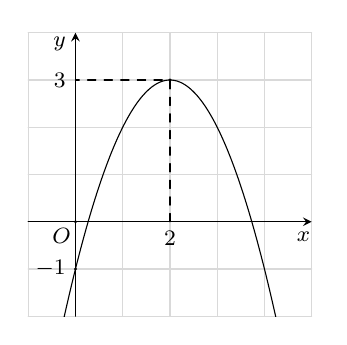
\begin{tikzpicture}[scale=0.6,>=stealth,line join=round,line cap=round,font=\footnotesize]
			% Định nghĩa khung
			\def\xmin{-1} 
			\def\xmax{5}
			\def\ymin{-2} 
			\def\ymax{4} 
			% Vẽ hệ trục
			\draw [gray!30] (\xmin,\ymin)grid (\xmax,\ymax);
			\draw [->] (\xmin,0)--(\xmax,0) node [below, xshift=-3pt] {$x$};
			\draw [->] (0,\ymin)--(0,\ymax) node [left, yshift=-4pt] {$y$};
			\fill [black] (0,0) circle (1pt) node [xshift=-5pt,yshift=-5pt] {$O$};
			% Cắt hình
			\clip (\xmin,\ymin) rectangle (\xmax,\ymax);
			\def\f{-(\x-2)^2+3}
			% Vẽ đồ thị các hàm số
			\draw [smooth, samples=100] plot [domain=\xmin:\xmax] (\x, {\f});
			\fill (0,-1) circle (1pt) node [left] {$-1$}
			(2,3) circle (1pt)
			;
			\draw [dashed](2,0) node [below] {$2$}--(2,3)--(0,3) node [left] {$3$};
		\end{tikzpicture}
	}
	\loigiai{
		\begin{itemchoice}
			\itemch Vì parabol có bề lõm hướng xuống nên $a<0$. 
			\itemch Đồ thị hàm số cắt trục tung tại điểm có tung độ $c$ nên $c=-1$. 
			\itemch Hàm số đã cho đồng biến trên khoảng $(-\infty;2)$. 
			\itemch Thay $c=-1$ ta có hàm số $f(x)=ax^2+bx-1$. \\
			Vì đồ thị hàm số có tọa độ đỉnh $(2;3)$ nên ta có hệ phương trình 
			$$\heva{&-\dfrac{b}{2a}=2 \\ &a \cdot 2^2+b \cdot 2-1=3} \quad  \text{hay} \quad \heva{&4a+b=0 \\ &4a+2b=4}.$$
			Giải hệ ta được $a=-1$ và $b=4$. \\
			Do đó $f(x)=-x^2+4x-1$. \\
			Vậy $f(10)=-10^2+4 \cdot 10-1=-61$. 
		\end{itemchoice}
	}
\end{ex}
\begin{ex}%[Dự án đề cương 3 khối 10-11-12 Dot 3 -Truong Tuong]
	Một vận động viên tennis đánh bóng dọc sân, vị trí bóng chạm vợt cách mặt lưới $2$ m. Độ cao (đơn vị: m) của quả bóng (so với mặt sân) trong quá trình từ lúc chạm vợt đến khi rơi chạm mặt sân được mô tả bởi hàm số $$h=-0{,}06x^2+0{,}3x+0{,}6$$
	trong đó $x$ (m) là khoảng cách từ vị trí quả bóng đến mặt lưới.
	\choiceTF 
	{\True Quả bóng có độ cao $0{,}6$ m lúc chạm vợt}
	{\True Nếu mặt lưới cao $0{,}9$ m thì quả bóng sẽ bay qua lưới}
	{Độ cao lớn nhất của quả bóng là $0{,}96$ m}
	{\True Khoảng cách (tính theo phương dọc sân) giữa vị trí bóng chạm vợt đến khi bóng rơi chạm mặt sân là $6{,}53$ m (kết quả làm tròn đến hàng phần trăm)}
	\loigiai{
		\begin{itemchoice}
			\itemch Lúc quả bóng chạm vợt (tức khi $x=0$) thì độ cao quả bóng là $h(0)=0{,}6$ (m). 
			\itemch Có $h(2)=0{,}96>0{,}9$ nên quả bóng sẽ bay qua lưới. 
			\itemch Đồ thị hàm số $h$ có tọa độ đỉnh là $(2{,5};0{,}975)$ nên độ cao lớn nhất của quả bóng là $0{,}975$ m. 
			\itemch Khi bóng rơi chạm mặt sân thì $h=0$ nên $-0{,}06x^2+0{,}3x+0{,}6=0$. \\
			Giải phương trình ta được $x \approx 6{,}53$. \\
			Vậy khoảng cách (tính theo phương dọc sân) giữa vị trí bóng chạm vợt đến khi bóng rơi chạm mặt sân là $6{,}53$ m.
		\end{itemchoice}
	}
\end{ex}
\Closesolutionfile{ans}
%\inputansbox[2]{2}{ans/answer.tex}

\begin{center}
	\textbf{PHẦN 3 - CÂU TRẮC NGHIỆM TRẢ LỜI NGẮN}
\end{center}
\setcounter{ex}{0}
\Opensolutionfile{ans}[ans-KQ-ONTAPCHUONG-DE1]
\begin{ex}%[Dự án đề cương 3 khối 10-11-12 Dot 3 -Truong Tuong]
	Cho hàm số bậc hai $y=ax^2+bx+c$ có đồ thị cắt trục hoành tại hai điểm phân biệt có hoành độ lần lượt là $-4$ và $3$. Tìm phương trình trục đối xứng của đồ thị hàm số đã cho. Viết kết quả dưới dạng số thập phân.
	\shortans{$-0,5$}
	\loigiai{
		Theo tính đối xứng của đồ thị hàm số bậc hai, ta có phương trình trục đối xứng của đồ thị hàm số đã cho là $x=\dfrac{-4+3}{2}=-0{,}5$. 
	}
\end{ex}
\begin{ex}%[Dự án đề cương 3 khối 10-11-12 Dot 3 -Truong Tuong]
	Giá bán lẻ điện sinh hoạt được cho trong bảng sau 
	\begin{center}
		\begin{tabular}{|>{\centering\arraybackslash}p{6cm}|>{\centering\arraybackslash}p{5cm}|}
			\hline
			Mức tiêu thụ (kW\,h) & Giá bán điện (đồng/kW\,h) \\
			\hline
			Bậc 1 (từ $0$ đến $50$) & $1\;678$ \\
			\hline
			Bậc 2 (từ trên $50$ đến $100$) & $1\;734$ \\
			\hline
			Bậc 3 (từ trên $100$ đến $200$) & $2\;014$ \\
			\hline
			Bậc 4 (từ trên $200$ đến $300$) & $2\;536$ \\
			\hline
			Bậc 5 (từ trên $300$ đến $400$) & $2\;834$ \\
			\hline
			Bậc 6 (từ $400$ trở lên) & $2\;927$ \\
			\hline
		\end{tabular}
	\end{center}
	Gọi hàm số $C(x)$ (đơn vị: nghìn đồng) biểu thị số tiền gia đình anh Hùng phải trả khi tiêu thụ hết $x$ kW\,h. Tính $C(325)$. Viết kết quả làm tròn đến hàng đơn vị.
	\shortans[oly]{$696$}
	\loigiai{
		Khi $x=325$, tức là gia đình anh Hùng tiêu thụ hết số kW\,h ở các bậc: $1$, $2$, $3$, $4$ và $25$ kW\,h ở bậc $5$. \\ 
		Như vậy số tiền gia đình anh Hùng phải trả là 
		$$C(325)=50 \cdot 1\,678+50 \cdot 1\,734+100 \cdot 2\,014+100 \cdot 2\,536+25 \cdot 2\,834=696\,450 \; \text{(đồng)} \approx 696 \; \text{(nghìn đồng)}.$$  
	}
\end{ex}
\begin{ex}%[Dự án đề cương 3 khối 10-11-12 Dot 3 -Truong Tuong]
	Cho hàm số $y=-\dfrac{4}{9}x^2+(2a-1)x-b$ với $a$, $b$ là các số thực. Biết đồ thị hàm số đã cho có tọa độ đỉnh là $(-1;4)$. Tính $a+b$. Viết kết quả dưới dạng số thập phân.
	\shortans[oly]{$-3,5$} 
	\loigiai{
		Đồ thị hàm số đã cho có tọa độ đỉnh $(-1;4)$ nên ta có hệ phương trình 
		$$\heva{&\dfrac{9(2a-1)}{8}=-1 \\ &-\dfrac{4}{9} \cdot (-1)^2+(2a-1) \cdot (-1)-b=4} \quad \text{hay} \quad \heva{&a=\dfrac{1}{18} \\ &b=-\dfrac{32}{9}.}$$
		Vậy $a+b=\dfrac{1}{18}-\dfrac{32}{9}=-3{,}5$.
	}
\end{ex}
\begin{ex}%[Dự án đề cương 3 khối 10-11-12 Dot 3 -Truong Tuong]
	Một vận động viên bóng rổ thực hiện cú ném bóng từ vị trí vòng tròn giữa sân cách rổ theo phương ngang $12,8$ m. Bóng được ném ở vị trí cao $2,5$ m và lọt vào rổ cao $3$ m. Khi đó quỹ đạo quả bóng là đường parabol có phương trình 
	\[y=-\dfrac{g}{2v_{0}^2\cos^{2}\alpha}x^2+x\tan\alpha+h\]
	với $y$ (m) là độ cao của quá bóng so với mặt sàn, $x$ (m) là khoảng cách quả bóng bay được theo phương ngang tính từ mặt đất tại vị trí ném, $g \; (\text{m/s}^2)$ là gia tốc trọng trường, $v_{0}$ (m/s) là vận tốc ban đầu và $\alpha$ là góc ném (góc tạo với phương ngang). Tính độ cao lớn nhất của quả bóng rổ trong quá trình bay biết rằng góc ném bằng $45^\circ$. Viết kết quả đơn vị m và làm tròn đến hàng phần trăm. \\
	\centerline{
		\begin{tikzpicture}[scale=.35,>=stealth,line join=round,line cap=round,font=\footnotesize]
			\def\a{15} 
			\def\k{28/15}
			\def\A{40} 
			\def\g{20} 
			\def\h{\a/5} 
			\path (0,0) coordinate (A)
			++(\g:\a) coordinate (B)
			($(A)!1!-\A:(B)!1-\k!(A)$) coordinate (D)
			++($(B)-(A)$) coordinate (C)
			($(A)!-.16!(B)!-.05!(D)$) coordinate (A')
			($(D)!-.16!(C)!-.09!(A)$) coordinate (D')
			($(B)!-.1!(A)!-.05!(C)$) coordinate (B')
			($(C)!-.1!(D)!-.09!(B)$) coordinate (C')
			($(A)!.5!(C)$) coordinate (boy);
			% Mặt ngoài sân
			\fill [black!90]
			(A')--++(-90:.3)--++($(D')-(A')$)--(D')--cycle
			(D')--++(-90:.3)--++($(C')-(D')$)--(C')--cycle;
			\draw [black!50,fill=orange!90!black!60] (A')--(B')--(C')--(D')--cycle;
			% Đường kẻ mặt sân
			\draw [white,line width=1pt] 
			\foreach \x/\y/\z in {A/B/0,D/C/180}{
				($(\x)!1/12!(\y)$) .. controls +(\z+\g-\A:{.7*\a}) and +(\z+\g-\A:{.7*\a}) .. ($(\x)!11/12!(\y)$)
			}
			\foreach \x/\y/\z/\t in {A/B/D/0,D/C/A/180}{
				($(\x)!.3!(\y)$)--++($.1*(\y)+.2*(\z)-.3*(\x)$)--++($.2*(B)-.2*(A)$)--($(\y)!.3!(\x)$)
				($(\x)!.3!(\y)$)++($.1*(\y)+.2*(\z)-.3*(\x)$) .. controls +(\t+\g-\A:{.15*\a}) and +(\t+\g-\A:{.15*\a}) .. ++($.2*(\y)-.2*(\x)$)
			}
			($(A)!.5!(D)$)--++($(B)-(A)$)
			($(A)!.5!(D)$)++($.38*(B)-.38*(A)$) .. controls +(\g-\A:{.15*\a}) and +(\g-\A:{.15*\a})
			.. ++($.24*(B)-.24*(A)$)
			.. controls +(180+\g-\A:{.15*\a}) and +(180+\g-\A:{.15*\a}) .. ++($.24*(A)-.24*(B)$);
			\draw [line width=1pt] (A)--(B)--(C)--(D)--cycle;
			% Bảng gần
			\draw [fill=gray!5] ($(D)!.4!(C)$)++(90:.9*\h)--++($.2*(B)-.2*(A)$)--++(90:.7*\h)--++($.2*(A)-.2*(B)$)--cycle;
			\draw [red!60,line width=.8pt] ($(D)!.45!(C)$)++(90:\h)--++($.1*(B)-.1*(A)$)--++(90:.35*\h)--++($.1*(A)-.1*(B)$)--cycle;
			% 2 Trụ
			\fill [red!60!black!80] ($(A)!.45!(B)$)--($(A)!.55!(B)$)--++(90:.3*\h)--++($1/30*(A)-1/30*(B)+(90:.2*\h)$)--++(90:.3*\h)--++($1/30*(A)-1/30*(B)$)--++(-90:.3*\h)--++($1/30*(A)-1/30*(B)+(-90:.2*\h)$)--++(-90:.3*\h)
			($(D)!.45!(C)$)--($(D)!.55!(C)$)--++(90:.3*\h)--++($1/30*(A)-1/30*(B)+(90:.2*\h)$)--++(90:.6*\h)--++(135+\g-\A:.02*\a)--++($1/30*(A)-1/30*(B)$)--++(\g-\A-45:.02*\a)--++(-90:.6*\h)--++($1/30*(A)-1/30*(B)+(-90:.2*\h)$)--++(-90:.3*\h);
			% Bảng xa
			\draw [fill=gray!5] ($(A)!.4!(B)$)++(90:.8*\h)--++($.2*(B)-.2*(A)$)--++(90:.7*\h)--++($.2*(A)-.2*(B)$)--cycle;
			\draw [red,line width=.8pt] ($(A)!.44!(B)$)++(90:.95*\h)--++($.1*(B)-.1*(A)$)--++(90:.35*\h)--++($.1*(A)-.1*(B)$)--cycle;
			% Rổ
			\fill [pattern=crosshatch,pattern color=gray!30] ($(A)!.5!(B)+(180:.03*\a)$)++(90:\h) 
			.. controls +(-60:\h/6) and +(110:\h/6) .. ++(-80:\h/3)--($(A)!.5!(B)+(0:.03*\a)+(90:\h)+(-100:\h/3)$)
			.. controls +(60:\h/6) and +(-110:\h/6) .. ($(A)!.5!(B)+(0:.03*\a)+(90:\h)$)
			arc (0:180:{.03*\a} and {.02*\a});
			\draw [gray!50] ($(A)!.5!(B)+(180:.03*\a)$)++(90:\h) 
			.. controls +(-60:\h/6) and +(110:\h/6) .. ++(-80:\h/3)
			($(A)!.5!(B)+(0:.03*\a)+(90:\h)+(-100:\h/3)$)
			.. controls +(60:\h/6) and +(-110:\h/6) .. ($(A)!.5!(B)+(0:.03*\a)+(90:\h)$);
			\draw [red,line width=.8pt] ($(A)!.5!(B)$)++(90:\h) ellipse ({.03*\a} and {.02*\a});
			% Boy
			\begin{scope}[scale=.35]
				% Chân
				\draw [fill=orange!20] (boy)++(-1.19, 0.93) 
				.. controls +(-0.08, 0.77) and +(-0.26, -0.48) .. ++(-0.21, 2.54)
				.. controls +(-0.37, 2.28) and +(-0.40, 0.21) .. ++(0.82, 1.43)
				.. controls +(-0.03, -0.37) and +(0.29, 0.82) .. ++(-0.32, -1.48)
				.. controls +(0.21, -0.66) and +(-0.03, 0.69) .. ++(0.00, -2.25)--cycle
				(boy)++(0.66, 1.22) .. controls +(0.03, 0.85) and +(-0.08, -0.82) .. ++(-0.37, 2.33)
				.. controls +(-0.71, 1.77) and +(-0.32, 0.32) .. ++(.42, 1.27)
				.. controls +(0,-1.03) and +(.16,2.01) .. ++(.34,-3.55)--cycle
				% Tay trái
				(boy)++(-1.48,9.71) .. controls +(-.08,.66) .. ++(0,.87)
				.. controls +(-.61,1.35) and +(-.34,-.66) .. ++(-.61,2.62)
				.. controls +(.08,.21) and +(.32,-.19) .. ++(-.32,.74)
				.. controls +(-.13,.08) and +(-.32,.26) .. ++(.24,-.05) 
				.. controls +(-.37,.34) and +(-.24,.37) .. ++(.03,.13) coordinate (t)
				.. controls +(-.05,.32) and +(-.16,.62) .. ++(.24,-.05)
				.. controls +(.03,.32) and +(-.08,.4) .. ++(.21,-.08)
				.. controls +(-.03,-1.16) and +(-.53,.87) .. ++(.63,-2.59)
				.. controls +(.24,-.11) .. ++(.37,-.42)
				.. controls +(-.34,-.61) and +(-.03,-.66) .. cycle
				(boy)++(.9,9.32) .. controls +(.42,.74) and +(.56,0) .. ++(-.11,1.19)
				.. controls +(-1.06,0) .. ++(-1.51,1.01)
				.. controls +(-.13,.24) and +(.16,-.19) .. ++(-.19,.63)
				.. controls +(0,.29) and +(-.13,.48) .. ++(-.08,-.19)
				.. controls +(-.24,.24) and +(-.26,.21) .. ++(-.08,-.11)
				.. controls +(-.45,.32) and +(-.4,.26) .. ++(.05,-.24) 
				.. controls +(-.48,.16) and +(-.21,.21) .. ++(.08,-.26) 
				.. controls +(.24,-.26) and +(-.66,.19) .. ++(.98,-1.11)--cycle;
				\draw [fill=orange!20]  (boy)++(-.37,11.96) .. controls +(-.63,-.74) and +(-.4,-.48) .. ++(.37,-1.22)
				.. controls +(-.34,.16) and +(.48,.19) .. ++(-.4,.74)
				.. controls +(.19,.19) and +(-.05,-.21) .. cycle;
				%
				%Tóc 
				\draw [fill=black] (boy)++(0,10.74) .. controls +(-.34,.16) and +(.48,.19) .. ++(-.4,.74)
				.. controls +(.19,.19) and +(-.05,-.21) .. ++(.03,.48) 
				.. controls +(.16,-.05) and +(.08,-.26) .. ++(.08,.21) 
				.. controls +(1.24,.53) and +(1.43,.19) .. cycle;
				% Giày
				\draw [fill=cyan] (boy)++(-1.30, .19) 
				.. controls +(-.16, 1.11) and +(-.05, -.53) 
				.. ++(.21, 1.14)--++(.48,-.27)--++(-.2,-1)--cycle
				(boy)++(0.45, 0.53) .. controls +(0.21, 0.45) and +(0.16, 0.69) .. ++(0.69, -0.08)
				.. controls +(.08,.58) .. ++(.03,.77) 
				.. controls +(-.19,.4) and +(.29,.37) .. ++(-.63,-.03) 
				.. controls +(0,-.24) .. cycle
				;
				\draw [fill=brown](boy)++(-1.30,.19) 
				.. controls +(.03,-.42) and +(.24, -.66) .. ++(.61,.37)
				.. controls +(.29,.21) and +(.37,.26) .. ++(-.13,.42)
				.. controls +(-.24,-.11) and +(.5,.11) .. cycle
				(boy)++(0.45, 0.53) .. controls +(0.21, 0.45) and +(0.16, 0.69) .. ++(0.69, -0.08)
				.. controls +(-0.29, -0.08) and +(0.13, -0.08) .. ++(-0.69, 0.08)
				;
				% Áo
				\draw [fill=red!80!black!60] (boy)++(-1.85,4.87) .. controls +(.74,-.19) .. ++(1.43,0)
				.. controls +(-.03,.32) .. ++(0,.66)
				.. controls +(.16,-.34) .. ++(.26,-.71)
				.. controls +(.11,.19) and +(-.05,-.24) .. ++(1.14,.08)
				.. controls +(-.16,.74) and +(.58,-.69) .. ++(-.56,2.62)
				.. controls +(-.26,-.13) and +(.61,-.08) .. ++(-1.83,-.16)
				.. controls +(-.45,-.37) and +(-.29,.4) .. ++(-.24,-1.53)
				.. controls +(-.11,-.53) .. cycle;
				\draw [fill=red!90!black!50] (boy)++(.42,7.51) .. controls +(-.26,-.13) and +(.61,-.08) .. ++(-1.83,-.16)
				.. controls +(-.08,1.01) and +(-.16,-.98) .. ++(-.08,2.35)
				.. controls +(-.03,-.66) and +(-.34,-.61) .. ++(.69,1.16)
				.. controls +(.08,-.08) and +(0,-.13) .. ++(.24,.11)
				.. controls +(.19,-.26) and +(-.32,-.13) .. ++(.87,-.32) 
				.. controls +(.13,-.11) .. ++(.4,-.16)
				.. controls +(.26,-1.11) and +(.21,.79) .. ++(-.13,-2.12)
				.. controls +(.16,-.34) and +(.21,.29) .. cycle;
			\end{scope}
			\draw [blue, line width=1pt,dashed] (t) .. controls +($.15*(A)-.15*(D)+(90:2*\h)$) and +($.15*(D)-.15*(A)+(90:2*\h)$) .. ($(A)!.5!(B)+(90:\h)$) coordinate [pos=.1] (t1) coordinate [pos=.5] (t2);
			\path (t1) coordinate (br);
			\begin{scope}[scale=.125]
				\fill [ball color= orange!100!brown] (br) circle (3);
				\fill [orange!30!black!100] (br)++(1.89,2.28) .. controls +(-1.25,1.05) and +(-.18,2.95) .. ++(-4.49,-3.7)
				.. controls +(.09,2.32) and +(-1.68,1) .. cycle;
				\fill [orange!30!black!100] (br)++(-2.45,1.67) .. controls +(.73,-1.25) and +(-1.94,.41) .. ++(4.71,-3.58)
				--++(-.1,-.11) .. controls +(-1.37,.1) and +(.92,-1.72) .. ++(-4.7,3.56)--cycle;
				\fill [orange!30!black!100] (br)++(-.95,2.81) .. controls +(-2.38,-2.59) and +(-.63,1.64) .. ++(3.92,-2.78)
				.. controls +(-.87,1.32) and +(-2.78,-2.57) .. cycle;
				\fill [orange!30!black!100] (br)++(-2.94,.34) .. controls +(1.06,.4) and +(-1.48,1.08) .. ++(2.73,-3.3)
				.. controls +(-1.32,.2) and +(1,.34) .. ++(-2.74,3.14)--cycle;
			\end{scope}
			\path (t2) coordinate (br);
			\begin{scope}[scale=.125]
				\fill [ball color= orange!100!brown] (br) circle (3);
				\fill [orange!30!black!100] (br)++(1.89,2.28) .. controls +(-1.25,1.05) and +(-.18,2.95) .. ++(-4.49,-3.7)
				.. controls +(.09,2.32) and +(-1.68,1) .. cycle;
				\fill [orange!30!black!100] (br)++(-2.45,1.67) .. controls +(.73,-1.25) and +(-1.94,.41) .. ++(4.71,-3.58)
				--++(-.1,-.11) .. controls +(-1.37,.1) and +(.92,-1.72) .. ++(-4.7,3.56)--cycle;
				\fill [orange!30!black!100] (br)++(-.95,2.81) .. controls +(-2.38,-2.59) and +(-.63,1.64) .. ++(3.92,-2.78)
				.. controls +(-.87,1.32) and +(-2.78,-2.57) .. cycle;
				\fill [orange!30!black!100] (br)++(-2.94,.34) .. controls +(1.06,.4) and +(-1.48,1.08) .. ++(2.73,-3.3)
				.. controls +(-1.32,.2) and +(1,.34) .. ++(-2.74,3.14)--cycle;
			\end{scope}
			\draw [<->,violet] ($(A)!.5!(B)+(-90:.02*\a)$)--($(A)!.5!(C)$) node [midway,sloped,fill=white,inner sep=1pt] {\bf 12,8};
			\draw [<->,violet] ($(A)!.5!(B)+(-90:.1*\h)$)--($(A)!.5!(B)+(90:\h)$) node [midway,sloped,fill=white,inner sep=1pt] {\bf 3};
			\path ($(A)!-.08!(B)$)--++($(D)-(A)$) node [midway,sloped,black,scale=.5] {\sffamily \bf TRUONG TUONG};
			\draw [<->,violet] ($(A)!.5!(D)+.6*(B)-.6*(A)$)--++(90:1.55*\h) node [midway,sloped,fill=white,inner sep=1pt] {\bf 2,5};
		\end{tikzpicture}
	}
	\shortans[oly]{$5,83$}
	\loigiai{
		Thay $h=2{,}5$ và $\alpha=45^\circ$ ta có $y=-\dfrac{g}{v_0^2}+x+2{,5}$. \\
		Đặt $a=-\dfrac{g}{2v_0^2}$, hàm số trở thành $y=ax^2+x+2{,}5$. \\
		Đồ thị hàm số đi qua điểm $(12{,}8;3)$ nên 
		$$a \cdot (12{,}8)^2+12{,}8+2{,}5=3 \quad \text{hay} \quad a=-\dfrac{615}{8192}.$$
		Suy ra $y=-\dfrac{615}{8192}x^2+x+2{,}5$. \\
		Độ cao lớn nhất của quả bóng xấp xỉ $5{,}83$ m. 
	}
\end{ex}
\Closesolutionfile{ans}

\begin{center}
	\textbf{PHẦN 4 - TỰ LUẬN}
\end{center}
\setcounter{ex}{0}
\begin{ex}%[Dự án đề cương 3 khối 10-11-12 Dot 3 -Truong Tuong]
	Tìm tập xác định của hàm số $y=\sqrt{2x-3}+\dfrac{5}{x-4}$. 
	\loigiai{
		Hàm số đã cho xác định khi $2x-3 \ge 0$ và $x-4 \neq 0$ hay $x \ge \dfrac{3}{2}$ và $x \neq 4$. \\
		Vậy tập xác định $\mathscr{D}=\left[\dfrac{3}{2};+\infty\right) \setminus \{4\}$. 
	}
\end{ex}
\begin{ex}%[Dự án đề cương 3 khối 10-11-12 Dot 3 -Truong Tuong]
	Một quả đạn pháo được bắn ra từ nòng của một khẩu pháo đặt cách mặt đất $2$ m, vận tốc ban đầu $100$ m/s, góc bắn $60^\circ$. Khi đó độ cao (đơn vị: m) của quả đạn pháo (so với mặt đất) được cho bởi hàm số 
	$$y=-0{,}00196x^2+1{,}732x+2$$
	trong đó $x$ (đơn vị: m) là tầm xa của quả đạn (tham khảo hình bên dưới). 
	\begin{listEX}[1]
		\item Quả đạn pháo bay xa được tối đa bao nhiêu m thì độ cao của nó bắt đầu giảm?
		\item Quả đạn pháo bay xa nhất bao nhiêu m?
	\end{listEX}
	\centerline{
		\begin{tikzpicture}[scale=0.6,>=stealth,line join=round,line cap=round,font=\footnotesize]
			\path 
			(0,0) coordinate (O)
			(0,1) coordinate (ph)
			(5,0) coordinate (ph1);
			\fill [gray] (-3,0) rectangle (13,-1);
			\draw (0,1) .. controls +(20:5) and +(150:4) .. ++(12,-1) node [starburst,fill=gray!50,scale=.3,line width=.3] {\bf BÙM}
			\foreach \x in {0,...,3}{
				coordinate [pos=\x/4] (boom\x)
			};
			\foreach \x in {0,...,3}{
				\begin{scope}[scale=.1]
					\fill [ball color=gray] (boom\x) circle (1);
					\fill [gray] (boom\x)++(-.2,.9)--++(90:.2) arc (180:360:{.2} and {.1})--++(-90:.2) arc (0:-180:{.2} and {.1});
					\draw [gray,line width=.2](boom\x)++(90:1.1) .. controls +(-.3,.5) and +(.3,0) .. ++(-1,-.3);
					\fill [black!60] (boom\x)++(90:1.1) ellipse ({.2} and {.1});
				\end{scope}
			}
			\begin{scope}[scale=.145]
				\draw [fill=black] (ph)++(-.13,.45)--++(-.24,-.05) .. controls +(-.19,.45) and +(-.03,.45) .. ++(-.66,-.13)--++(-.32,-.08)
				.. controls +(-.08,.24) and +(-.13,.29) .. ++(-.26,-.08)--++(-9.74,-2.25)
				.. controls +(-.05,.19) and +(-.11,.24) .. ++(-.21,-.05)--++(-.26,-.05)
				.. controls +(-.08,.29) and +(-.08,.24) .. ++(-.24,-.08)
				.. controls +(-.37,-.03) and +(.13,.26) .. ++(-.66,-.56)
				.. controls +(0,-.4) and +(.19,.05) .. ++(-.58,-.13)
				.. controls +(-1.08,-.08) and +(-.97,-.48) .. ++(.32,-1.15)
				.. controls +(.19,.05) and +(-.2,.34) .. ++(.57,.18)
				.. controls +(.25,-.16) and +(-.33,-.17) .. ++(.85,-.14)
				.. controls +(.05,-.25) and +(.08,-.29) .. ++(.25,.05)--++(.25,.09)
				.. controls +(.03,-.26) and +(.05,-.19) .. ++(.21,.06)--++(9.53,3.01)
				.. controls +(.03,-.32) and +(.05,-.25) .. ++(.27,.07)--++(.31,.09)
				.. controls +(.21,-.4) and +(.07,-.48) .. ++(.64,.22)--++(.23,.08)--cycle;
				\foreach \y in {-11.91,-7.86}{
					\fill [black] (ph)++(\y,-6.06) circle (1.04);
					\foreach \x in {1,...,6}{
						\fill [white] (ph)++(\y,-6.06)--++({20+(\x-1)*60}:.69) arc ({20+(\x-1)*60}:{65+(\x-1)*60}:.69);
					}
					\fill [black] (ph)++(\y,-6.06) circle (.38);
					\fill [white] (ph)++(\y,-6.06) circle (.21);
				}
				\draw [line width=.2,white,fill=black] (ph)++(-10.16,-3.87) .. controls +(-.07,.5) and +(.4,-.03) .. ++(-.58,-.68)
				.. controls +(-.56,-.13) and +(.95,.45) .. ++(-.77,-.98)--++(0,-.58)--++(3.31,0)
				.. controls +(.16,.58) and +(-.11,-.74) .. ++(-.37,1.75)
				.. controls +(.03,.19) and +(.18,-.04) .. ++(-.16,.49)
				.. controls +(.26,1.33) and +(-.26,1.33) .. cycle;
				\fill [white] (ph)++(-9.445,-3.6) circle (.4);
				\fill (ph)++(-9.445,-3.6) circle (.2);
			\end{scope}
			\draw [<->] (0,1)--(0,0) node [midway,fill=white,inner sep=1pt] {$2$};
			\draw [<->] (boom1)--($(O)!(boom1)!(ph1)$) node [pos=.5, fill=white, inner sep=.5pt] {$y$};
			\draw [<->] ($(O)!(boom1)!(ph1)$)++(-90:.3)--(0,-.3) node [pos=.5, fill=white, inner sep=.5pt] {$x$};
			\draw [->] (0,1)--++(25:2);
			\draw [dashed] (0,1)--++(2,0);
			\draw (0,1)++(1,0) arc (0:25:1) node [midway,right,yshift=1pt] {$60^\circ$};
		\end{tikzpicture}
	}
	\loigiai{
		\begin{listEX}[1]
			\item Độ cao của quả đạn tăng trong khoảng $\left(0;\dfrac{21\,650}{49}\right)$ và sau đó bắt đầu giảm. Như vậy, quả đạn pháo bay xa được tối đa $\dfrac{21\,650}{49} \approx 442$ (m) thì độ cao của nó bắt đầu giảm. 
			\item Vị trí xa nhất của quả đạn pháo sẽ nằm trên mặt đất nên $y=0$ hay $-0{,}00196x^2+1{,}732x+2=0$. \\
			Giải phương trình ta được $x \approx 885$. \\
			Vậy quả đạn pháo bay xa nhất $885$ m. 
		\end{listEX}
	}
\end{ex}
\begin{ex}%[Dự án đề cương 3 khối 10-11-12 Dot 3 -Truong Tuong]
	Một cửa hàng kinh doanh nhận thấy rằng: Nếu bán mỗi sản phẩm với giá $x$ triệu đồng thì mỗi ngày sẽ tiêu thụ được $100-5x$ sản phẩm, đồng thời chi phí bỏ ra (chi phí nhập hàng, thuê mặt bằng, thuê nhân công, $\cdots$) mỗi ngày là $C(x)=10x+200$ (triệu đồng). Hỏi lợi nhuận lớn nhất trong một ngày của cửa hàng là bao nhiêu triệu đồng? 
	\loigiai{
		Doanh thu mỗi ngày của công ty là $$x \cdot (100-5x)=100x-5x^2 \; \text{(triệu đồng)}.$$
		Lợi nhuận mỗi ngày của công ty là $$f(x)=100x-5x^2-(10x+200)=-5x^2+90x-200 \; \text{(triệu đồng)}.$$
		Đồ thị hàm số $y=f(x)$ có tọa độ đỉnh là $(9;205)$. \\
		Hàm số bậc hai $y=f(x)$ có hệ số $a=-5<0$ nên đạt giá trị lớn nhất bằng $205$, khi $x=9$. \\
		Vậy lợi nhuận lớn nhất trong một ngày của cửa hàng là $205$ triệu đồng. 
	}
\end{ex}